\section{SVM}

\subsection{Introduction}



\subsection{Methods}

In this part, we discuss some details about the implementation of SMO.


1. First, we normalized the training and test data. Then permutate the training data set by iterating over the patterns and swap the current one to a random position of the data set.  


2. In order to conduct 10-fold cross validation, we came up a training and validation set construction procedure over the permutated data set. The idea is that we divide the training set into ten equal-sized parts. For a specific setup of $C$ and $\tau$, the procedure sequentially extracts the i-th $(i=1,\cdots,10)$ part as the validation set and combines the other parts as the training set.

In each training loop, we maintain a binary index to efficiently update the set $I_{up}$ and $I_{low}$. Such binary index has the same number of entries as that of patterns in the training set. For instance, value $1$ in the $i$-th entry of $I_{up}$ index indicates the $i$-th pattern belongs to the set $I_{up}$. In this way, we only need to change the ownerships of the chosen violation pair. Then we invoke the max (or min) function of Matlab to get the most violated pair for next loop.   


\subsection{Results	$\&$ Discussion}

1.




\begin{table}[!h] 
	
 \centering\small
 \begin{threeparttable}
 \caption{\label{task1} \small Matrix of 10-fold CV scores\vspace{-5mm}
}
\vspace{-5mm}
  \begin{tabular}{lcccc}
  \toprule
           &$\tau=$ 0.02 & $\tau=$ 0.04 & $\tau=$ 0.06  & $\tau=$ 0.08 \\
  \midrule
   $C=4$ &1.613757  &0.902137  & 0.582406 & \textbf{0.406962} \\
$C=5$ & 1.655328 &0.901502 & 0.583424 & 0.407138\\
   $C=6$ &1.652844  &0.905430  & 0.583432 &0.407138\\
  $C=7$ &1.662291 &0.902036 & 0.583348 & 0.407138\\
  $C=8$ &1.674960 &0.906631 & 0.583348 & 0.407138\\
  \bottomrule
  \end{tabular}
 % 
 %  \small
 %  Note:
%  \begin{tablenotes}
%   \item[*] the best value of every metric in uniform model segmentation 
%  \end{tablenotes}
 \end{threeparttable}
% \footnotetext[1]{the best value of every metric in uniform model segmentation }
\end{table}

Based on the experience of program tuning, we set the domains of parameter $C$ and $\tau$ in $[4,8]$ and $[0.02,0.08]$ respectively to find the best configuration. In Tab. \ref{task1}, we present the matrix of 10-fold cross validation scores. We can see that the winning configuration is $C$=$4$ and $\tau$=$0.08$ which achieves the minimal CV score.


2.

\begin{figure}[htbp]
   \centering	
      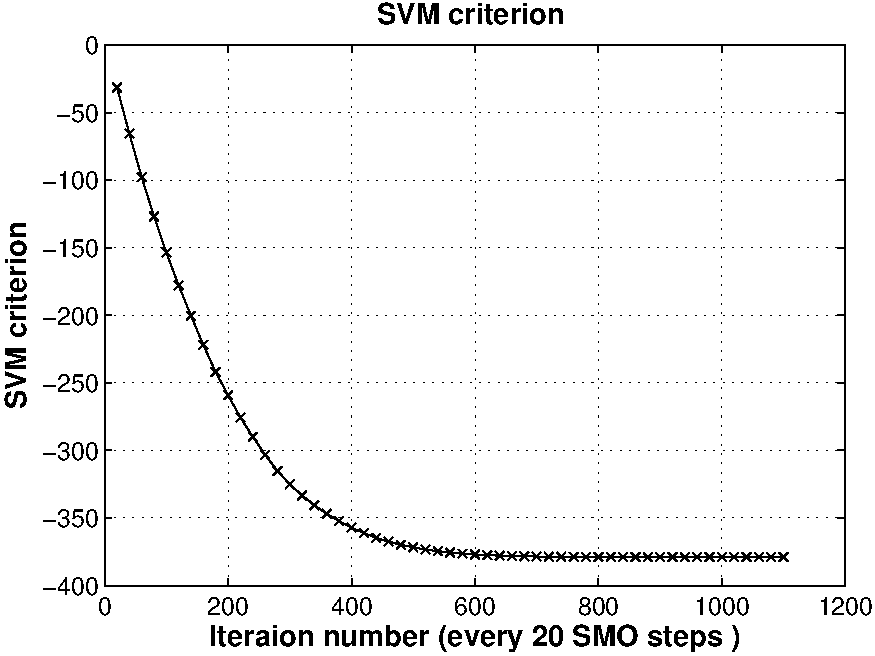
\includegraphics[width=10cm, height=4cm]{figs/task2-1.pdf} 	
%   \includegraphics[width=7.5cm, height=1.5cm]{figs/design/regsearch} 
   % \includegraphics[scale=0.2]{figs/tsch} 
   \vspace{-0.3cm}
   \caption{SVM criterion as a function of iteration number}\label{fig:task2-1}
   %\vspace{-0.5cm}
\end{figure}

\begin{figure}[htbp]
   \centering	
      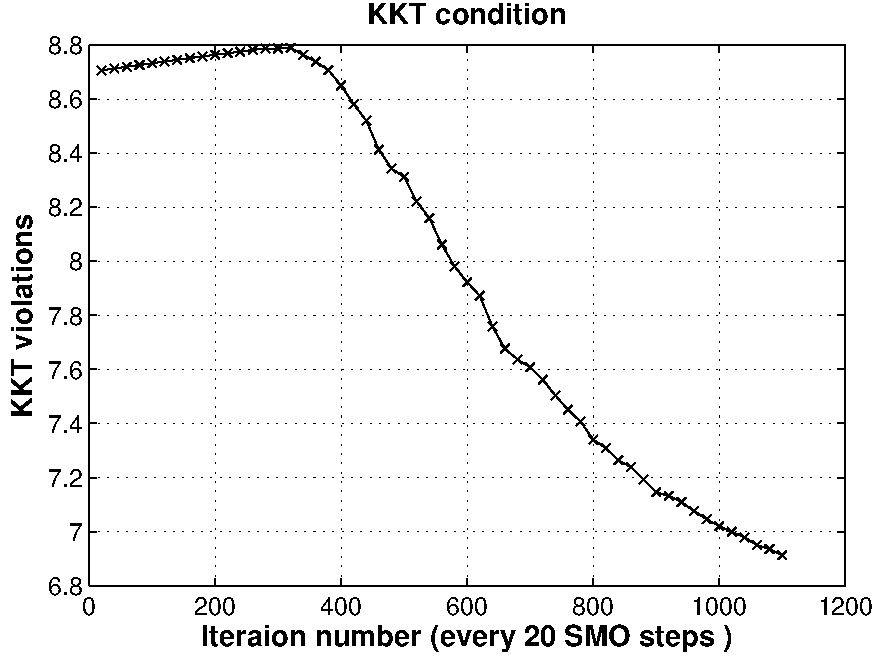
\includegraphics[width=10cm, height=4cm]{figs/task2-2.pdf} 	
%   \includegraphics[width=7.5cm, height=1.5cm]{figs/design/regsearch} 
   % \includegraphics[scale=0.2]{figs/tsch} 
   \vspace{-0.3cm}
   \caption{KKT violations as a function of iteration number}\label{fig:task2-2}
   %\vspace{-0.5cm}
\end{figure}


In this part, we run our SMO algorithm on the full training set, with the parameters found by above cross-validation. 


Fig. \ref{fig:task2-1} presents the decreasing trend of SVM criterion as a function of SMO iterations. After 600 iterations, the SVM criterion decreases slowly.

Fig. \ref{fig:task2-2} exhibits the variation of number of KKT condition violations in the training period. In the beginning phase, the KKT violations increases a little. This is because initially the set $I_0$ contains no patterns. Then when it has more elements, the violation number increases as the patterns in $I_0$ belong to both $I_{+}$ and $I_{-}$. 


3. In this experiment, we make use of the final SVM classifier trained by our SMO algorithm with the configuration from cross validation to perform on the whole training and test set. The zero/one error on training set is zero, while the misclassification rate for test set is $\frac{17}{1991}= 0.85\%$ 

4. In the last experiment, we compare the classification performance of the final MLP and SVM on both the training and test data. Fig. \ref{fig:task4} exhibits the results. We can see that the SVM outperforms the MLP on the training and test data sets. We leverage the Gaussian kernel which is an exponentially decaying function in the input feature space in SVM and therefore SVM works in a theoretically infinite feature space, which improves the separability of original data set. In the meanwhile, both MLP and SVM are more precise for training data than for test data. This is easy to understand, because the classifier are learnt from the training data with convergence threshold to ensure the precision. 


\begin{figure}[htbp]
   \centering	
      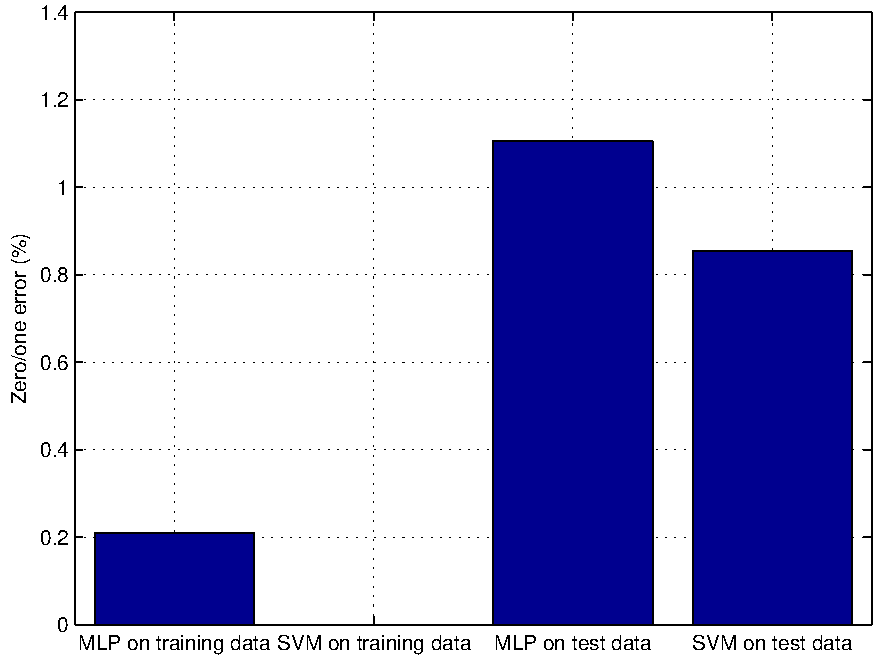
\includegraphics[width=6cm, height=4cm]{figs/task4.pdf} 	
%   \includegraphics[width=7.5cm, height=1.5cm]{figs/design/regsearch} 
   % \includegraphics[scale=0.2]{figs/tsch} 
   \vspace{-0.3cm}
   \caption{Comparison of zero/one errors of final MLP and SVM on training and test data sets}\label{fig:task4}
   %\vspace{-0.5cm}
\end{figure}

%finish on training set  6000 0 0.000000
%finish on test set  1974 17 0.008538


%finish on training set  0.000000
%finish on training set  0.007534

